\documentclass[12pt]{standalone}
\usepackage{fontspec}
\setsansfont{TeX Gyre Heros}
\newfontfamily\mfallback{DejaVu Sans}
\usepackage{tikz}
\usetikzlibrary{arrows.meta}
\begin{document}
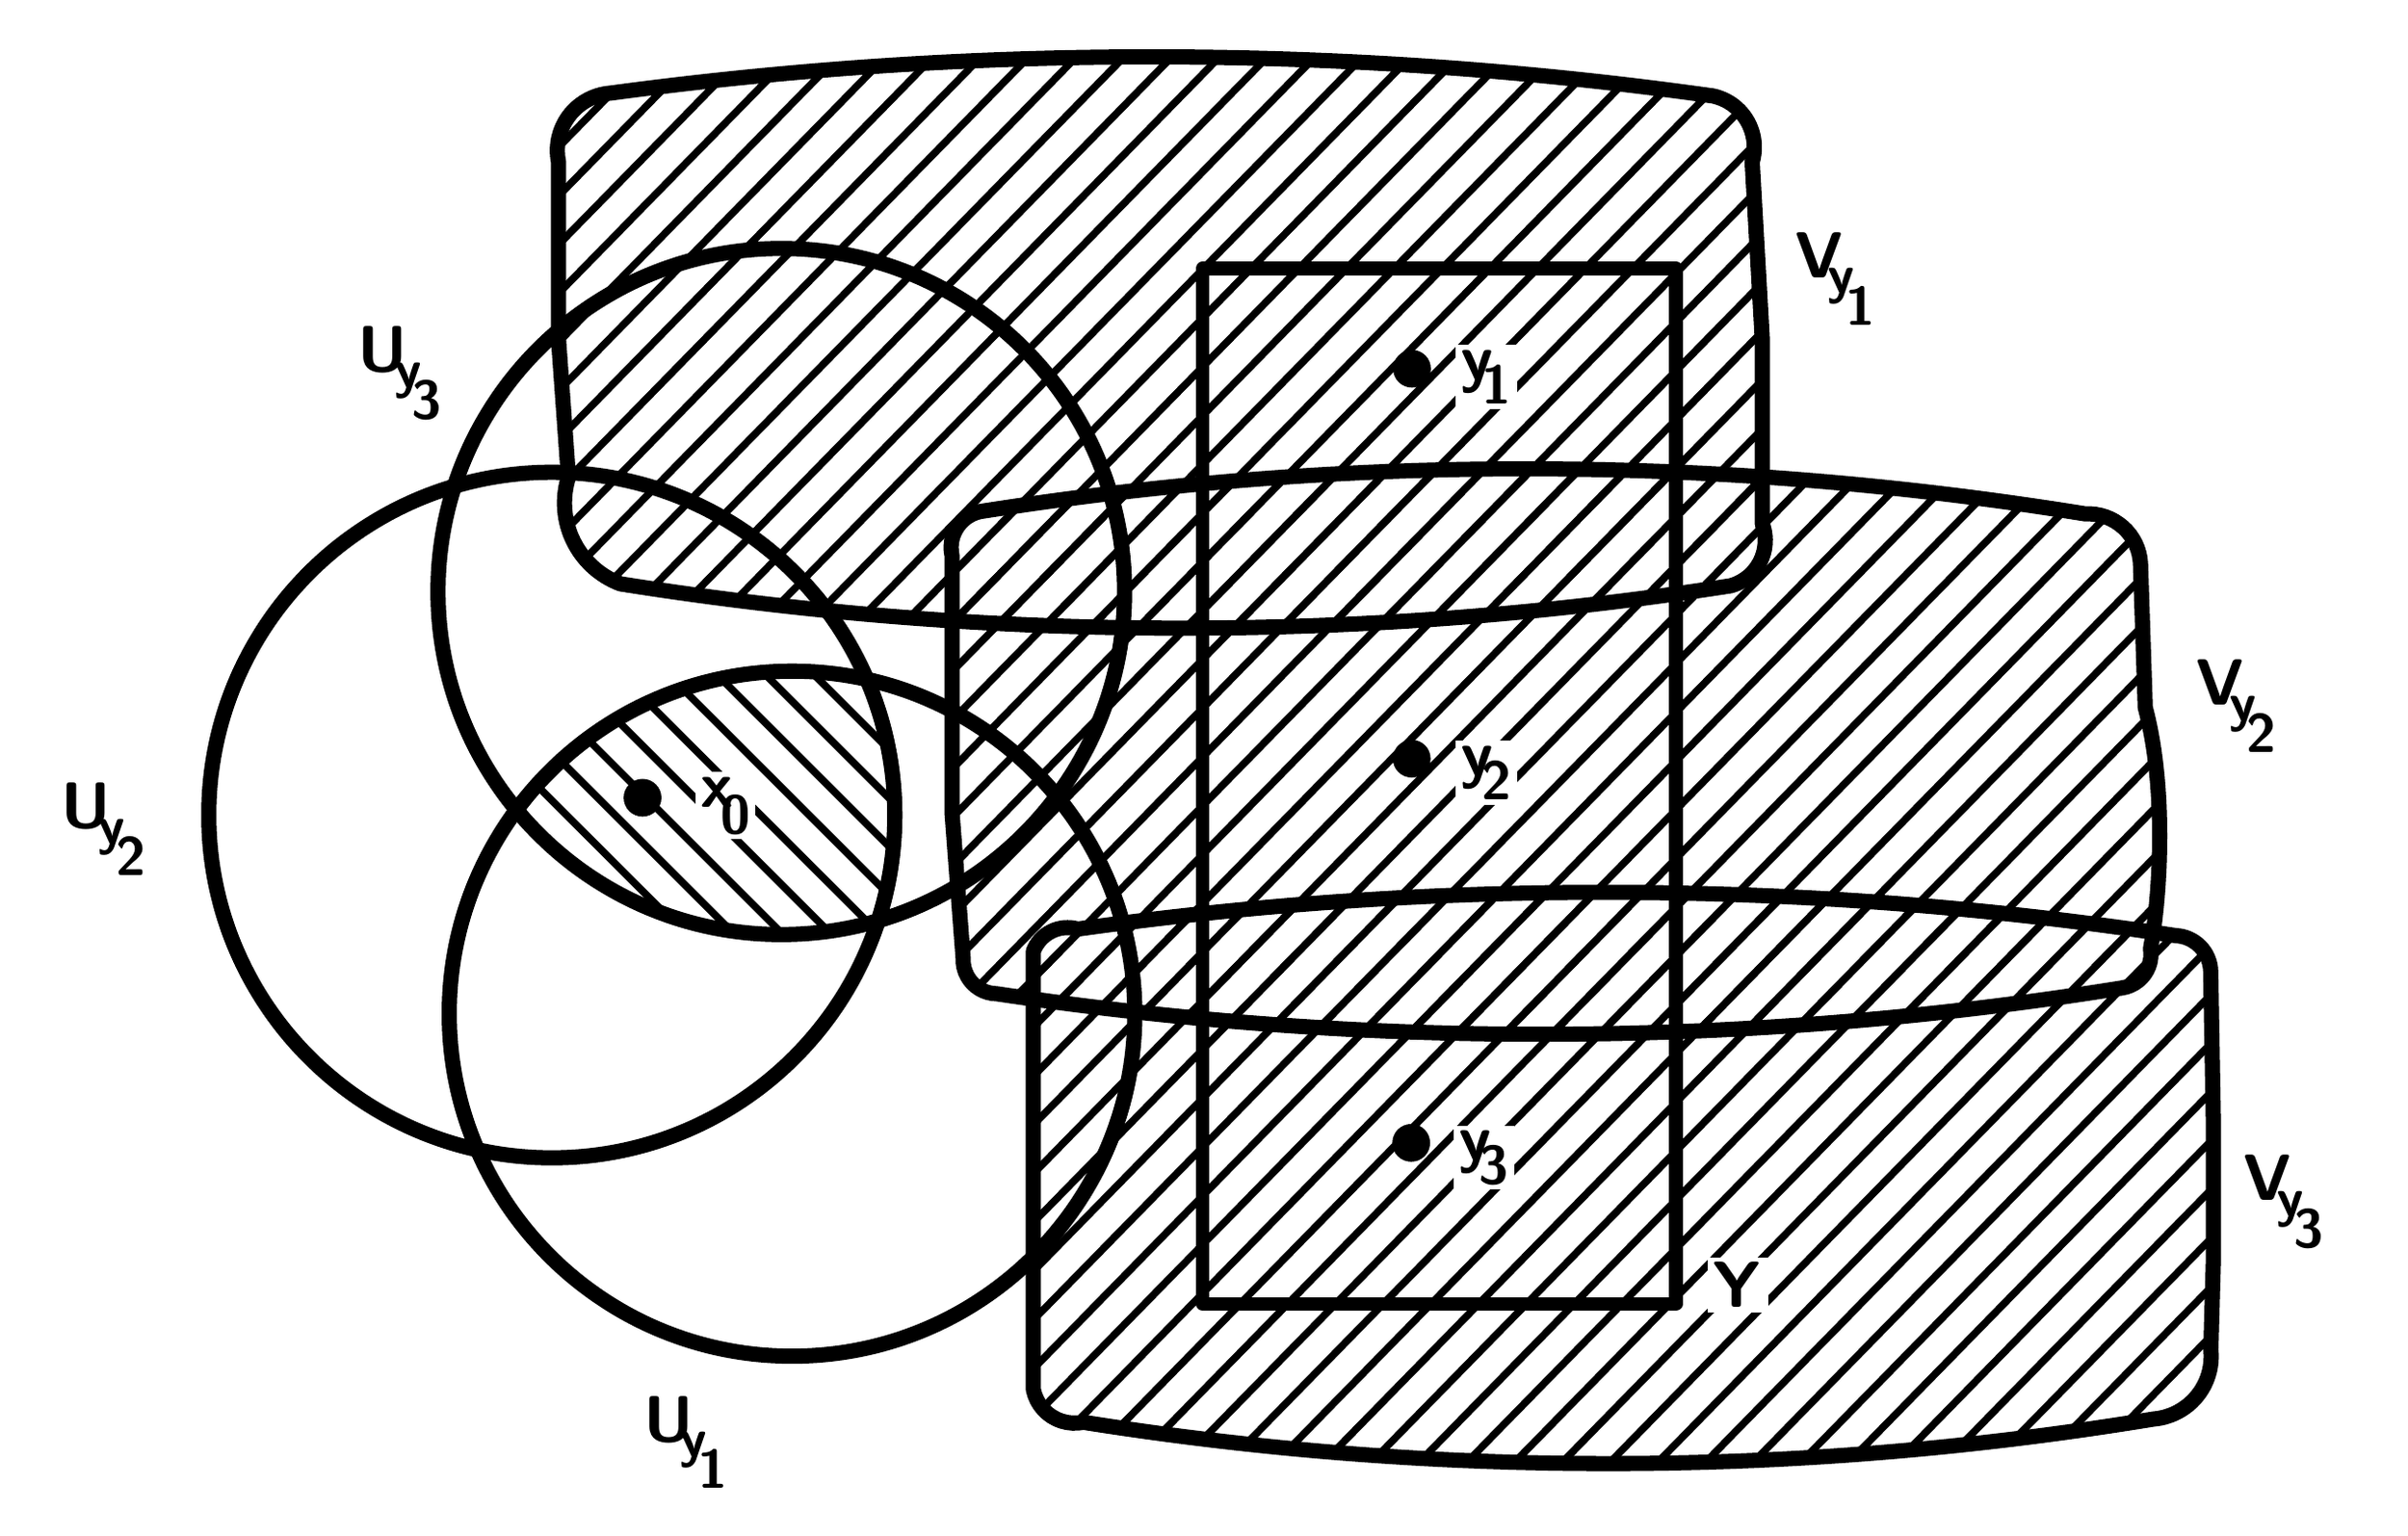
\begin{tikzpicture}[x=1pt, y=-1pt, line cap=round, line join=round]

  % ============================================================
  % 26.1 -- Y rectangle, three shaded open sets V_{y_i},
  % three circular neighbourhoods U_{y_i} of x0, common
  % intersection shaded (lens).
  % canvas: 898 x 566, 1pt = 1px, y down
  % ============================================================

  % ---------- the three V lobes (closed rounded shapes) --------
  % long edges and inner seams are circular arcs (centre/radius from
  % least-squares fits to the 600 dpi ink); corners are small arcs too.
  % V_{y1}: top lobe
  \def\VonePath{%
    (203,52)
    arc[start angle=168.06,end angle=266.03,radius=22]% TL corner
    arc[start angle=-97.67,end angle=-82.01,radius=1542.1]% top edge
    arc[start angle=-77.91,end angle=16.39,radius=20]% TR corner
    -- (662,120) -- (662,190)% right edge (scan sits ~4px right)
    arc[start angle=-20.08,end angle=74.19,radius=18]% BR corner
    arc[start angle=81.15,end angle=99.05,radius=1361.0]% bottom seam S1
    arc[start angle=110.76,end angle=197.35,radius=33]% BL corner
    -- (203,120) -- (203,52)}% left edge

  % V_{y2}: middle lobe
  \def\VtwoPath{%
    (353,202)
    arc[start angle=167.22,end angle=263.22,radius=14]% TL corner
    arc[start angle=-98.92,end angle=-80.78,radius=1332.9]% top seam S2
    arc[start angle=-92.95,end angle=-3.08,radius=20]% TR corner
    -- (808,260) .. controls (816,290) and (814,330) .. (810,352)% right edge (scan bulges ~7px)
    arc[start angle=-9.42,end angle=81.93,radius=13]% BR corner
    arc[start angle=80.88,end angle=98.53,radius=1398.3]% bottom seam S3
    arc[start angle=90.80,end angle=183.09,radius=13]% BL corner
    -- (353,300) -- (353,250) -- (353,202)}% left edge

  % V_{y3}: bottom lobe
  \def\VthreePath{%
    (384,353)
    arc[start angle=-159.32,end angle=-73.81,radius=14]% TL corner
    arc[start angle=-98.0,end angle=-81.33,radius=1444.2]% top seam S4
    arc[start angle=-87.15,end angle=-1.16,radius=14]% TR corner
    -- (834,420) -- (834,470) -- (833,505)% right edge
    arc[start angle=-6.15,end angle=85.55,radius=24]% BR corner
    arc[start angle=80.65,end angle=99.03,radius=1277.4]% bottom edge
    arc[start angle=77.98,end angle=168.28,radius=16]% BL corner
    -- (384,460) -- (384,400) -- (384,353)}% left edge

  % ---------- hatching (45 deg "/", common global phase) -------
  \newcommand{\hatchlines}{%
    \foreach \k in {-3,...,86}{%
      \pgfmathsetmacro{\cc}{11.5+18.2*\k}%
      \pgfmathsetmacro{\yA}{(\cc+120)/0.978}%
      \pgfmathsetmacro{\yB}{(\cc-1060)/0.978}%
      \draw[line width=2.8pt] (-120,\yA) -- (1060,\yB);%
    }%
  }

  % lens hatching: opposite direction (top-left to bottom-right, 45deg)
  \newcommand{\lenshatch}{%
    \foreach \k in {-8,...,4}{%
      \pgfmathsetmacro{\cc}{16+18.5*\k}%
      \draw[line width=2.8pt] (-120,{-120-\cc}) -- (1060,{1060-\cc});%
    }%
  }

  % shade the V union: each lobe clipped with the same global lines
  \begin{scope}\clip \VonePath;   \hatchlines\end{scope}
  \begin{scope}\clip \VtwoPath;   \hatchlines\end{scope}
  \begin{scope}\clip \VthreePath; \hatchlines\end{scope}

  % ---------- shaded lens = U_y1 cap U_y2 cap U_y3 -------------
  \begin{scope}
    \clip (287.9,215.7) circle (130.9);
    \clip (200.4,301.0) circle (130.8);
    \clip (292.0,376.8) circle (130.7);
    \lenshatch
  \end{scope}

  % ---------- V outlines (one closed path per lobe) ------------
  \draw[line width=5.8pt] \VonePath;
  \draw[line width=5.8pt] \VtwoPath;
  \draw[line width=5.8pt] \VthreePath;

  % ---------- Y : the rectangle --------------------------------
  \draw[line width=5.2pt] (448.5,92.5) rectangle (629,487.5);

  % ---------- circles U_y1, U_y2, U_y3 -------------------------
  \draw[line width=5.8pt] (287.9,215.7) circle (130.9);
  \draw[line width=5.8pt] (200.4,301.0) circle (130.8);
  \draw[line width=5.8pt] (292.0,376.8) circle (130.7);

  % ---------- marked points ------------------------------------
  \fill (528.4,130.7) circle (7.2);
  \fill (528.3,279.5) circle (7.2);
  \fill (528.1,426.1) circle (7.2);
  \fill (235.0,294.4) circle (7.2);

  % ---------- labels (one node each, white halo) --------------
  % U_{y3}
  \node[anchor=base west,inner sep=2.2pt,fill=white] at (124,132)
    {\fontsize{31}{37}\selectfont\textsf{\textbf{\textit{U}}}\kern-5pt%
     \raisebox{-6pt}{\fontsize{22}{26}\selectfont\textsf{\textbf{\textit{y}}}\kern-4pt%
       \raisebox{-12pt}{\fontsize{22}{26}\selectfont\textsf{\textbf{3}}}}};
  % U_{y2}
  \node[anchor=base west,inner sep=2.2pt,fill=white] at (11,306)
    {\fontsize{31}{37}\selectfont\textsf{\textbf{\textit{U}}}\kern-5pt%
     \raisebox{-6pt}{\fontsize{22}{26}\selectfont\textsf{\textbf{\textit{y}}}\kern-4pt%
       \raisebox{-12pt}{\fontsize{22}{26}\selectfont\textsf{\textbf{2}}}}};
  % U_{y1}
  \node[anchor=base west,inner sep=2.2pt,fill=white] at (233,540)
    {\fontsize{31}{37}\selectfont\textsf{\textbf{\textit{U}}}\kern-5pt%
     \raisebox{-6pt}{\fontsize{22}{26}\selectfont\textsf{\textbf{\textit{y}}}\kern-4pt%
       \raisebox{-12pt}{\fontsize{22}{26}\selectfont\textsf{\textbf{1}}}}};
  % V_{y1}
  \node[anchor=base west,inner sep=2.2pt,fill=white] at (672,96)
    {\fontsize{31}{37}\selectfont\textsf{\textbf{\textit{V}}}\kern-6pt%
     \raisebox{-6pt}{\fontsize{22}{26}\selectfont\textsf{\textbf{\textit{y}}}\kern-4pt%
       \raisebox{-12pt}{\fontsize{22}{26}\selectfont\textsf{\textbf{1}}}}};
  % V_{y2}
  \node[anchor=base west,inner sep=2.2pt,fill=white] at (825,259)
    {\fontsize{31}{37}\selectfont\textsf{\textbf{\textit{V}}}\kern-6pt%
     \raisebox{-6pt}{\fontsize{22}{26}\selectfont\textsf{\textbf{\textit{y}}}\kern-4pt%
       \raisebox{-12pt}{\fontsize{22}{26}\selectfont\textsf{\textbf{2}}}}};
  % V_{y3}
  \node[anchor=base west,inner sep=2.2pt,fill=white] at (843,448)
    {\fontsize{31}{37}\selectfont\textsf{\textbf{\textit{V}}}\kern-6pt%
     \raisebox{-6pt}{\fontsize{22}{26}\selectfont\textsf{\textbf{\textit{y}}}\kern-4pt%
       \raisebox{-12pt}{\fontsize{22}{26}\selectfont\textsf{\textbf{3}}}}};
  % y1
  \node[anchor=base west,inner sep=2.0pt,fill=white] at (545,135)
    {\fontsize{31}{37}\selectfont\textsf{\textbf{\textit{y}}}\kern-5pt%
     \raisebox{-9pt}{\fontsize{22}{26}\selectfont\textsf{\textbf{1}}}};
  % y2
  \node[anchor=base west,inner sep=2.0pt,fill=white] at (545,286)
    {\fontsize{31}{37}\selectfont\textsf{\textbf{\textit{y}}}\kern-5pt%
     \raisebox{-9pt}{\fontsize{22}{26}\selectfont\textsf{\textbf{2}}}};
  % y3
  \node[anchor=base west,inner sep=2.0pt,fill=white] at (544,433)
    {\fontsize{31}{37}\selectfont\textsf{\textbf{\textit{y}}}\kern-5pt%
     \raisebox{-9pt}{\fontsize{22}{26}\selectfont\textsf{\textbf{3}}}};
  % x0
  \node[anchor=base west,inner sep=2.0pt,fill=white] at (255,298)
    {\fontsize{31}{37}\selectfont\textsf{\textbf{\textit{x}}}\kern-5pt%
     \raisebox{-10pt}{\fontsize{22}{26}\selectfont\textsf{\textbf{0}}}};
  % Y
  \node[anchor=base west,inner sep=2.0pt,fill=white] at (641,489)
    {\fontsize{29}{35}\selectfont\textsf{\textbf{\textit{Y}}}};

  \pgfresetboundingbox
  \path[use as bounding box] (0,0) rectangle (898,566);
\end{tikzpicture}
\end{document}
